\documentclass[]{report}
\title{\textbf{Dossier de validation}\\Développeur Fullstack}
\author{Alexandre Rousseau}

\usepackage{graphicx}
\usepackage{hyperref}
\usepackage[utf8]{inputenc}
\usepackage[french]{babel}
\usepackage{appendix}
\usepackage{pdfpages}
\usepackage{listings}
\usepackage{csquotes}
\usepackage{lstautogobble}

\hbadness=99999
\hfuzz=999pt

\pagestyle{headings}

\hypersetup{
    colorlinks,
}

\begin{document}

\lstset{
  autogobble,% remove leading space indentation
  breaklines=true, % sets automatic line breaking
  captionpos=b, % sets the caption-position to bottom
  frame=single, % adds a frame around the code
  showtabs=false, % show tabs within strings adding particular underscores
  tabsize=2, % sets default tabsize to 2 spaces
}

\maketitle

\newpage

\tableofcontents
\newpage

\pagenumbering{arabic}

\chapter{Préface}

  \section{Remerciements}

    %TODO

  \section{Introduction}

    Dans le souhait de me former et de progresser continuellement, je me suis inscrit sur le site  \href{https://cofondateur.fr}{cofondateur.fr} . Ce réseau social met en relation des entrepreneurs qui cherchent des développeurs pour construire leurs idées. C'est ainsi que je suis rentré en contact avec une startup qui cherchait un profil technique pour la réalisation de leur projet.

    Cette expérience  m'a permis de sortir de ma zone de confort et ainsi de construire un projet de A à Z.

\chapter{Présentation du projet}



  Les deux cofondateurs sont Adrien ORION et Sacha PARTENSKY, deux étudiants en droit à l’université Lyon 3 Jean Moulin. Au stade de la rencontre, ils avaient créé la société et elle était suivie par un incubateur\footnote{un incubateur est une société externe qui aide à la création d'un startup}.

  \section{La société}

    La société fait partie des LegalTech\footnote{Une LegalTech peut se définir comme une startup de droit en ligne qui propose aux entreprises et aux particuliers une offre numérique} créée en tant que iSignif SAS. Il s'agit donc d'une Société par actions simplifiées. Ce type de société nous a permis de rédiger un pacte d'actionnaires et ainsi de partager les droits de décision équitablement.

    \begin{figure}
      
\includegraphics[width=\linewidth]{img/logo.png}
      \caption{Le logo d'iSignif}
    \end{figure}

    Quelques semaines plus tard, nous signions ensemble le nouveau pacte d'actionnaires. Nous redéfinissions ainsi les parts et les rôles des nouveaux associés:

    \begin{itemize}
      \item Adrien ORION, cofondateur et directeur général, associé à hauteur de 31,5\%
      \item Sacha PARTENSKY, cofondateur et Président à hauteur de 41,5\%
      \item Alexandre ROUSSEAU, CTO, associé à hauteur de 25\%
    \end{itemize}

    J'ai donc choisi un rôle de sociétaire car c'est compatible avec mon statut de salarié chez GAC Technology.

  \section{Statut juridique}

    % https://www.lecoindesentrepreneurs.fr/pourquoi-creer-une-sasu/

    La SASU\footnote{Société par Actions Simplifiée Unipersonnelle} est le statut privilégié. Les avantages de ce statut juridique sont:

    \begin{itemize}
      \item Responsabilité de l'associé unique limitée au montant de son apport
      \item Possibilité de nommer un DG assistant le Président associé-unique
      \item Montant minimal de capital social de 1 euro
      \item Régime social des assimilés-salariés pour le gérant = protection accrue et cotisations au prorata de la rémunération
    \end{itemize}

    L'inconvénient de ce statut est qu'il est plus difficile à mettre en place et qu'il faut rédiger tous les statuts par écrit. Dans notre cas, ce statut est parfait puisque mes associés ont les compétences pour rédiger les \textquote{formalités}.

  \section{Analyse du besoin}

    %% pompé sur plaquette invest.docx

    Réalisée par un huissier de justice, la signification a pour but de porter les actes judiciaires\footnote{assignation en justice, jugement, sommation de payer ou de faire, congés, demandes de renouvellement du bail commercial...} à la connaissance des intéressés. 

    Toutefois, les actes sont souvent adressés à plusieurs destinataires résidents dans des villes éloignées. Ceci demande un effort chronophage pour les demandeurs de signification qui doivent contacter les huissiers compétents pour chaque adresse (voir figure \ref{fig:signification_before}).

    \begin{figure}[h!]
      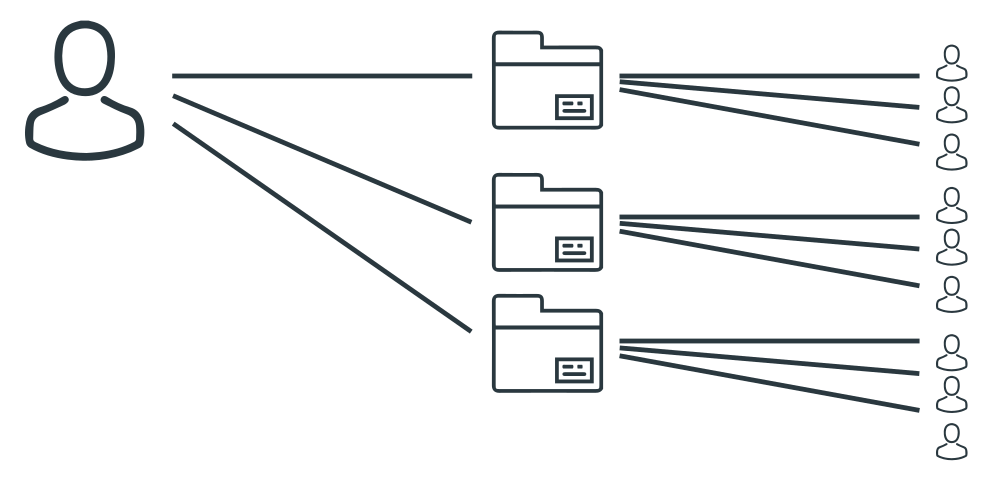
\includegraphics[width=\linewidth]{img/signification_before.png}
      \caption{Un acte doit être notifié en main propre pour chaque destinataire}
      \label{fig:signification_before}
    \end{figure}

    L'idée d'iSignif est donc de créer une plateforme afin de simplifier le processus de signification en centralisant les demandes et en les répartissant automatiquement vers un huissier compétent du réseau  (voir figure \ref{fig:signification_after}).

    \begin{figure}
      
\includegraphics[width=\linewidth]{img/signification_after.png}
      \caption{L'acte est centralisé et signifié à tous les destinataires}
      \label{fig:signification_after}
    \end{figure}

  \section{Business plan}

    La grande problématique de notre activité est que la loi interdit toute forme de publicité pour les huissiers. Il est donc important qu'on ne favorise pas certains huissier plutôt que d'autres. Nous avons donc choisit un système qui répartie par ordre d'arrivée les demande de significations.

    Notre modèle économique réside sur l'idée de facturer les huissiers en fonction du nombre d'affaire qu'on leur apporte. Pour faire cela, nous avons eu plusieurs idées:

    \begin{itemize}
      \item prendre une facturation mensuelle d'une somme fixée par nombre d'affaire apportés
      \item demander un abonnement qui donne le droit d'accéder au réseau
      \item proposer un système de \textquote{crédit} afin que les huissier pré-paye un nombre d'affaire qu'on va leur apporter
    \end{itemize}

    Dans un premier temps, nous avons choisis d'utiliser le système de facturation mensuel. Je vous reparlerais de l'impacte que cela a eu dans la section \ref{sec:feedback}.


  \section{Réalisation du cahier des charges}

    L'idée est donc de construire une plateforme qui centralise toutes les demandes. Ces demandes doivent être accessibles:

    \begin{itemize}
      \item à n'importe quel moment
      \item sur tout type de support (ordinateur, smartphone, tablette, etc..).
    \end{itemize}

    Il était donc naturel de se tourner vers une application web qui convient à ce besoin.

    Nous avons donc rédigé un premier cahier des charges. Ce premier de cahier des charges correspond à la version bêta qui sera proposée aux bêta testeurs. Cette version doit donc être fonctionnelle.

    \subsection{Système de connexion}

      Comme la plupart des sites web, la plateforme doit posséder un système de connexion. Nous devons pouvoir connaître l’identité de la personne qui navigue sur le site et interdire certaines fonctionnalités à certains types de comptes. Par exemple un huissier ne pourra pas créer d'actes à signifier.

    \subsection{Estimation du coût d'un acte}

      Il s'agit d'une des fonctionnalité les plus attractives pour l'avocat. Il doit pouvoir, en un minimum de clic, avoir une estimation du coup de son acte. Sachant que cette page sera le point d'entrée de l'application, elle doit être le plus simple possible. Cette page devra donc être en Single Page.

    \subsection{Création des factures}

      Afin d'éviter le stockage sur le serveur, nous avons pensé à stocker directement les informations des factures en base de données. Ainsi, la plateforme sera capable de générer des factures sous forme de fichier PDF directement à la demande. Cette méthode a néanmoins l'inconvénient d'utiliser plus de ressources car on peut générer plusieurs fois la même facture.

    \subsection{Parrainage}

      Les avocats peuvent choisir de travailler avec certains huissiers qui ne font pas partie du réseau iSignif. Ainsi, il leur sera possible d'inviter des huissiers externes à rejoindre le réseau.

    \subsection{Statistiques}

      % TODO

    \subsection{Administration}

      % TODO

  \section{Conceptualiser et modéliser les données}

    Lors de la rencontre avec les cofondateurs, nous avions échangé à propos des fonctionnalités de l'application. A la fin de la réunion, ils m'ont remis plusieurs documents dont une ébauche de cahier des charges.

    A mon sens, la suite logique était de valider la conception d'un modèle de donnée. Ceci permet de valider la compréhension de logique métier et la faisabilité du projet. De plus, cette étape m'a permis d'estimer le temps que le projet allait me coûter en terme de temps.

    J'ai donc choisi la méthode Merise que j'ai eu l'occasion de découvrir en cours à l'IT-AkAdemy. Bien que moins actuelle elle permet de réaliser un graphique compréhensible par des profils non-techniques.

    \subsection{Étude d'une partie du diagramme de modèle de données}

      \subsubsection{Les utilisateurs}

        Prenons par exemple la gestion des utilisateurs. Dans l'application il existe deux principaux types de comptes:

        \begin{itemize}
          \item les avocats qui peuvent faire la demande de signification d'un acte
          \item les huissiers qui peuvent signifier les demandes auxquelles ils sont affecté
        \end{itemize}

        Ces deux types de comptes possèdent les mêmes propriétés (nom, prénom, courriel, mot de passe). J'ai donc choisi de faire un héritage avec un modèle \verb|User|. Ainsi, les deux modèles partagent les mêmes propriétés (voir figure \ref{fig:merise_users}).

        \begin{figure}[h!]
          \centering
          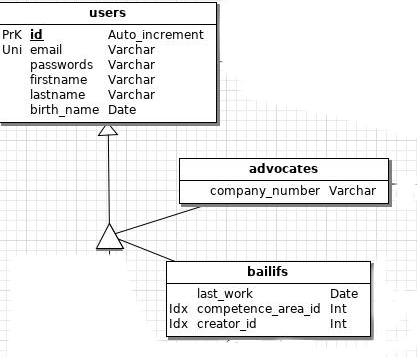
\includegraphics[width=0.5\textwidth]{img/merise_users.png}
          \caption{Représentation de l'héritage entre les huissiers et les avocats}
          \label{fig:merise_users}
        \end{figure}

        Concrètement dans une base de données relationnelles, cela se matérialisera par une \href{https://en.wikipedia.org/wiki/Single_Table_Inheritance}{Single Table Inheritance}. C'est-à-dire qu'une table contiendra les deux types de données et qu'une colonne spécifiera le type d'utilisateur (Huissier ou Avocat). Ce modèle d'héritage en architecture de base de données est assez controversé. Cependant il convient bien à mon cas car les deux entités sont quasiment identiques.

      \subsubsection{Les huissiers}

        Contrairement à l'avocat, l'huissier aura des relations supplémentaires avec d'autres entités. Chaque huissier est affecté à une unique zone de compétence. Cette zone de compétence contient plusieurs villes matérialisées sous l'entité \verb|zip_code|. Nous arrivons donc au résultat présenté sur la figure \ref{fig:merise_bailiffs}.

        \begin{figure}[h!]
          \centering
          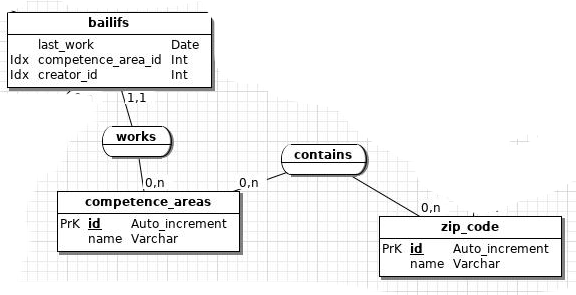
\includegraphics[width=0.8\textwidth]{img/merise_bailiffs.png}
          \caption{Représentation des huissiers}
          \label{fig:merise_bailiffs}
        \end{figure}

      \subsubsection{L'acte}

        Nous pouvons ensuite créer une nouvelle entité \verb|Act| qui représentera un acte qui devra être signifié par un huissier. Cet acte doit donc contenir:

        \begin{itemize}
          \item les avocats qui peuvent faire la demande de signification d'un acte
          \item les huissiers qui peuvent signifier les demandes auxquelles ils sont affectés
          % -- vérification lorène
        \end{itemize}

    \subsection{Résultats final}

      %% bailif here
      J'ai donc obtenu le résultat final que l'on peut voir sur la figure \ref{fig:merise_zoom} et le diagramme complet figure \ref{fig:merise}.

      \begin{figure}
        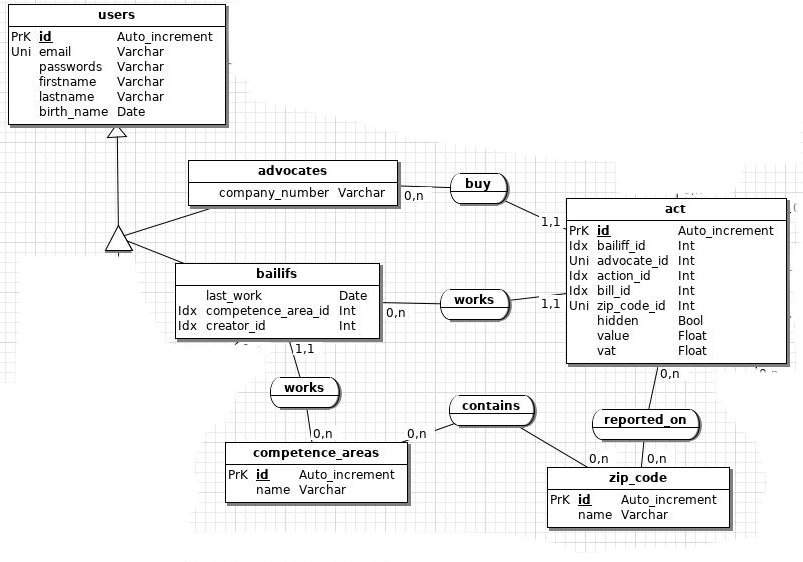
\includegraphics[width=\linewidth]{img/merise_zoom.png}
        \caption{ébauche de la première version du diagramme Merise réalisé avec jMerise en mai 2018}
        \label{fig:merise_zoom}
      \end{figure}

      Une fois le diagramme validé, j'ai pu commencer les spécifications techniques de l'application.

      \begin{figure}
        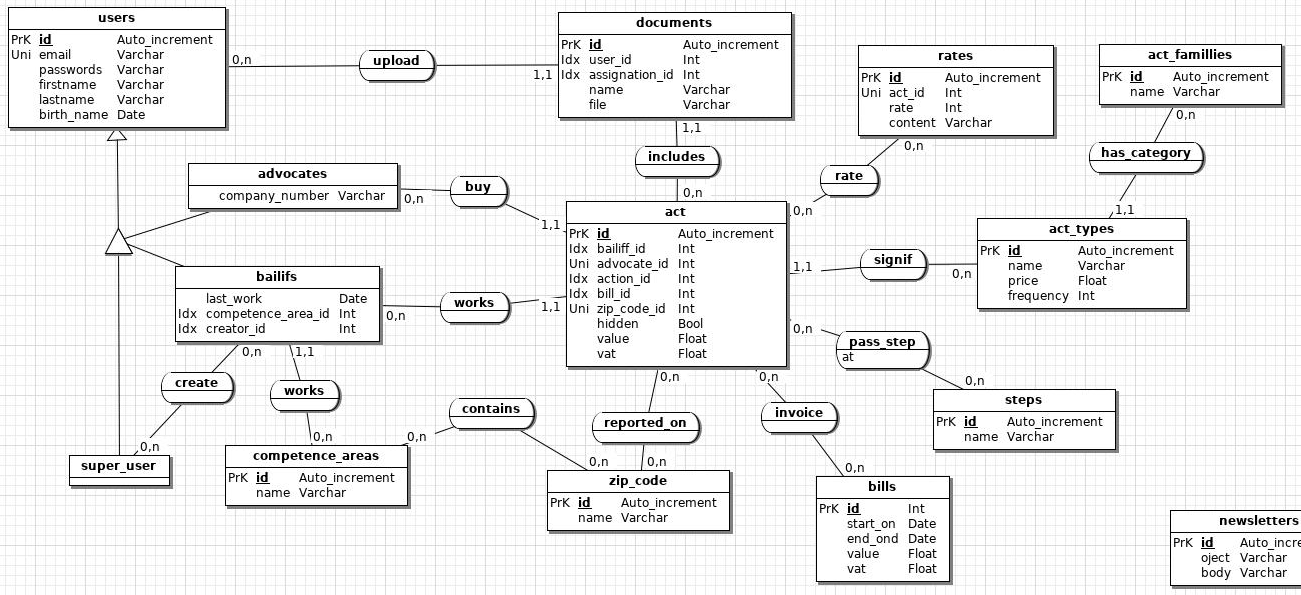
\includegraphics[width=\linewidth]{img/merise.png}
        \caption{Première version du diagramme Merise réalisé avec jMerise en mai 2018}
        \label{fig:merise}
      \end{figure}

\chapter{Planifier la réalisation du projet}

  \section{Réunions d'avancements}

    Les réunions d'avancements ont lieu physiquement. Elles ne sont pas périodiquement fixées, nous en organisons à la demande, lorsqu'un membre de l'équipe en ressent le besoin. Nous en faisons donc une tous les mois environ d'une heure ou deux. Afin d'être plus efficace, nous définissons un but à l'avance.

    L'idée n'est donc pas de développer une \textquote{réunionite} mais bien de valider certaines étapes du développement du produit et de communiquer autour de l'avancé de la société.

    Voici donc quelques réunions clés qui se sont déroulées au cours de l'élaboration de notre produit.

    \subsection{Présentation de la première version}

      Cette réunion a eu lieu le 30 mai 2017, c'est à dire quelques semaines après ma rencontre avec les cofondateurs. A ce moment là, j'avais travaillé en total autonomie sur l'élaboration d'un produit fonctionnel.

      L'objectif était donc de valider les \textquote{fondations} de cette plateforme. Cette étape est réellement importante. Je devais savoir que cette première ébauche correspondait aux attentes des deux cofondateurs.

      J'ai donc effectué une démonstration. Cela a permis de renforcer la confiance que mes associés m'avaient alors accordé mais aussi de collecter des premières critiques.

    \subsection{Rencontre des incubateurs}

      Cette réunion à eu lieu le 6 juin 2016 et nous a permis de rédiger le pacte des associés.

      Le projet était incubé par \href{Beelys}{https://www.beelys.org/}, un grand incubateur lyonnais. Beelys nous offrait donc l'aide de deux spécialistes en startups. Ces spécialistes nous on apporté des renseignements sur le fonctionnement des levées de fond.

      A la suite de cette réunion, nous avons fait le choix de mettre de côté la levée de fond. En effet, une levée de fond s'accorde souvent d'une vente de part de l'entreprise. Sachant que nous n'avions pas besoin immédiatement d'argent', nous préférions garder les parts de l'entreprise et les vendre une fois que la société posséderait une certaine notoriété.

    \subsection{Présentation de l’outil à un huissier}

      Cette réunion a eu lieu le 12 septembre. A ce moment, le produit était presque prêt pour le lancement en bêta.

      L'huissier avait participé en tant que bêta testeur pour un de nos concurrent le plus aboutit. Cela a permit de collecter les retours qu'il avait eu et de les intégrer à notre application. Cela nous a aussi permis de valider notre produit et d'apporter quelques petites corrections avant le lancement.

  \section{Méthode Kanban}

    La méthode Kanban est méthode agile très utilisée dans le monde informatique. Cela permet de mettre en place une gestion du projet sous forme de tickets. Cela permet de visualiser le flux de travail, de limiter le nombre de tâches en cours et de prioriser les tâches.

    Cette méthode nous était indispensable car elle permet de voir l'avancement du projet sans nous \textquote{surcharger} de réunions.

    Dans un premier temps je n'ai pas choisi de d'utiliser la méthode AGILE et la gestion des Sprints. Pour nous, le premier livrable devait être la phase bêta. Cette phase devrait correspondre à un produit fonctionnel en se concentrant sur les fonctions basiques.

    \subsection{Découpage des tâches}

      Nous avons donc fait une réunion autour de laquelle nous avons découpé toutes les tâches à réaliser. Chaque tâche doit donc:

      \begin{itemize}
        \item être indivisible
        \item réalisable rapidement
      \end{itemize}

      \paragraph{Colonne \textquote{à faire (bêta)}}

        Nous avons donc très rapidement sélectionné les tâches qui devaient être réalisé obligatoirement avant le lancement de la bêta. C'est à dire:

        \begin{itemize}
          \item indispensable au \textit{workflow} du client
          \item à fore valeur ajoutée en terme de marketing
          \item développable rapidement
          \item générique aux besoins des différents clients
        \end{itemize}

      \paragraph{Colonne \textquote{à faire"}}

        Cette colonnes réunit les tâches qui seront nécessaires après le déploiement de la bêta.

      \paragraph{Colonne \textquote{idées}}

        Comme le nom l'indique, cette colonne peut réunir toutes les idées d'amélioration ou de mise en place de fonctionnalité.

    \subsection{Utilisation de Trello}

      Dans le monde du Kanban, un logiciel SAAS se démarque parmi les autre: \href{http://trello.com/}{Trello}. Trello est un outil SAAS qui permet pousse la méthode Kanban plus loin. Cette application pousse la collaboration en ajoutant les discussions sur les tâches (voir figure \ref{fig:trello}).

      \begin{figure}
        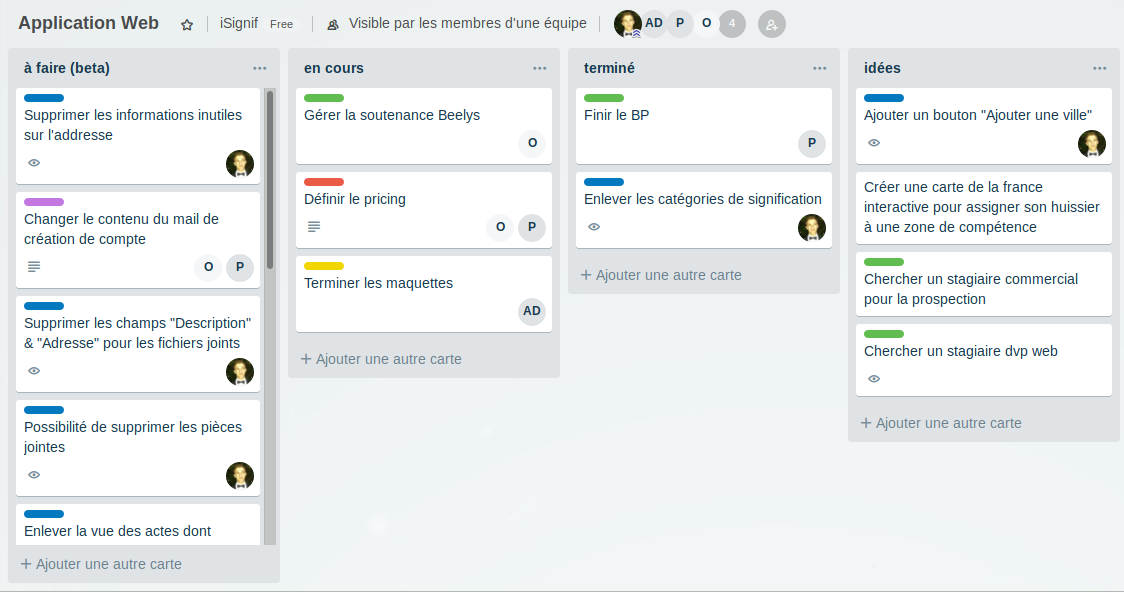
\includegraphics[width=\linewidth]{img/trello.png}
        \caption{Capture d'écran de notre tableau Kanban en septembre 2018}
        \label{fig:trello}
      \end{figure}

      Première version bêta pour septembre 2018

  \section{Rédiger les spécifications techniques}

    Étant dans une équipe non technique, mes associés m'ont laissé carte blanche pour le choix des technologies. Les seule contraintes étaient de respecter un développement rapide et fiable. Si l'on considère la représentation figure \ref{fig:good_cheap_fast}, je devais donc me situer entre \textit{good} et \textit{cheap}.

    \begin{figure}
      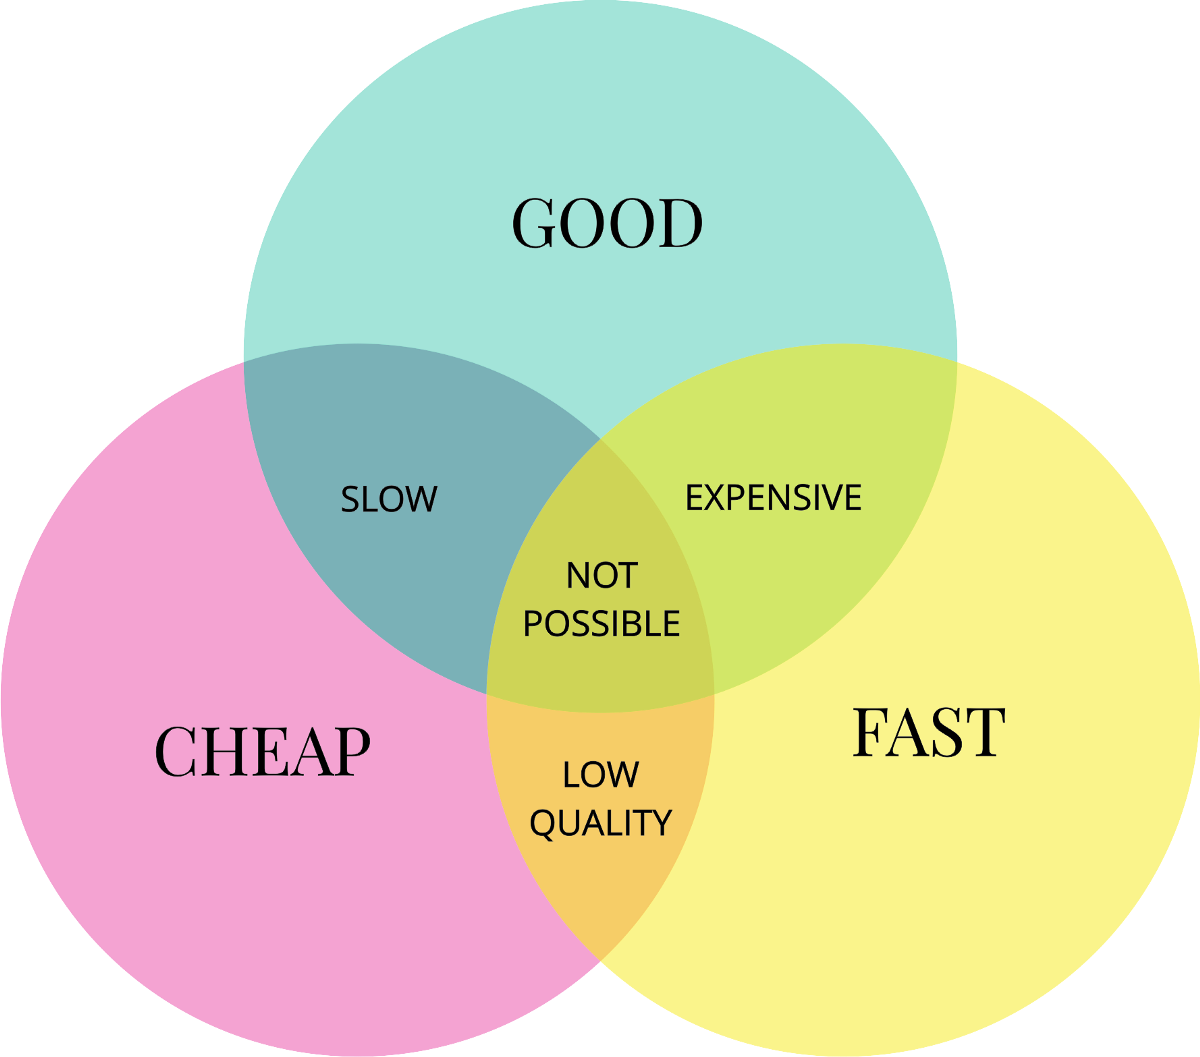
\includegraphics[width=0.5\textwidth]{img/good_cheap_fast.png}
      \caption{Un bon résumé du choix à faire lors de l'élaboration des spécification techniques}
      \label{fig:good_cheap_fast}
    \end{figure}


    \subsection{Back-end}

      Étant donné que dans un premier temps je serais le seul à développer le produit, mon objectif était de choisir un framework ou j'étais à l'aise. Mon choix c'est donc naturellement posé sur \href{https://rubyonrails.org/}{Ruby on Rails}.

      \href{https://rubyonrails.org/}{Ruby on Rails} est un framework web écrit en \href{Ruby}{https://www.ruby-lang.org/}. Très utilisé dans le monde des startup\footnote{ Ruby on Rails a été initialement utilisé pour \href{https://github.com/}{Github}, \href{https://twitter.com/}{Twitter}, \href{https://airbnb.com/}{Airbnb}, \href{https://soundcloud.com/}{Soundcloud}, etc.. .}, sa grande force est une grande communauté et une très bonne maturité. Par son mantra \textit{"Convetion over configuration"}\footnote{"Suivez les convention au lieu de configurer"}, il permet un développement extrêmement rapide.

    \subsection{Front-end}

      Les nouvelles applications utilisent des interface utilisateurs de plus en plus réactive. La tendance étant aux \textit{Signle Page Application}\footnote{Application sur une page}, j'ai choisis de rester plus simple dans un premier temps.

      J'ai néanmoins choisis de mettre en place Vue.JS, un \textit{framework front-end} pour designer les pages qui demandent le plus d’interactions. J'ai choisis Vue.JS au lieu de React ou Angular car c'est le plus simple à mettre en place.

    \subsection{MariaDB}

      %TODO

  \section{Travailler à plusieurs}\label{sec:git}

    Git\footnote{Git est un logiciel développé par Linux Torvals (fondateur de Linux) qui permet de versionner un projet. Ainsi il rend la collaboration beaucoup plus facile.} est énormément utilisé dans le monde du développement de logiciel. Son efficacité n'est plus à prouver. Pour construire iSignif, j'ai immédiatement décidé d'appliquer la méthodologie \textbf{Git Flow}.

    \begin{figure}
      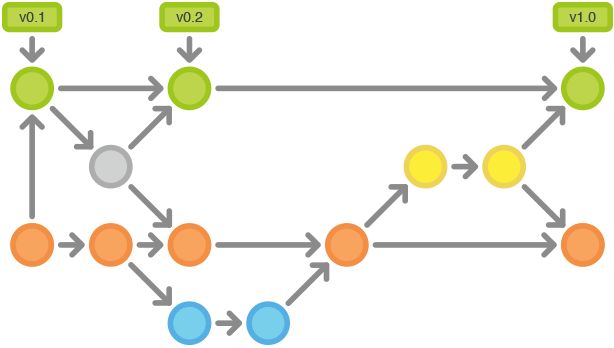
\includegraphics[width=\linewidth]{img/git-flow.png}
      \caption{Schéma du \textit{workflow} de Git Flow.}
      \label{fig:git-flow}
    \end{figure}

    Git Flow impose une convention de travail avec Git (voir figure \ref{fig:git-flow}). Sur ce schéma, on retrouve:

    \begin{description}
      \item[en vert] la branche \verb|master| correspond à l'état actuel de l'application en production.
      \item[en rouge] la branche \verb|develop| contient tous les nouveaux développement qui seront publié lors de la prochaine mise en production.
      \item[en bleu] cela correspond à une \verb|feature|, c'est à dire une fonctionnalité développé indépendamment de l'application.
      \item[en jaune] il s'agit d'une \verb|release|, c'est à dire une mise en publication de tous les développement validés.
      \item[en gris] Il s'agit d'un \verb|hotfix|. Ce sont des petits correctifs fait à la fois sur la branche \verb|master| et \verb|develop|.
    \end{description}

    Cette méthodologie permet ainsi de travailler à plusieurs sans se géner puisque chaque développeur peut travailler indépendamment sur une branche \verb|feature|. De plus, ceci me permet de faire des mise en production régulièrement (j'en parlerai plus en détails dans la section \ref{sec:deployments}).

\chapter{Développement de la plateforme}

  \section{Développement Dirigé par les Test}\label{sec:tdd}

    Etant le seul développeur \textit{back-end}, il m'a fallut m'organiser afin d'optimiser au maximum mon temps.

    De mon point de vue, une des façon d'optimiser son développement est d'assurer ses arrières afin d'éviter de corriger des bogues. Pour cela, ma solution est les tests unitaires\footnote{Les test unitaires sont du code qui permet de vérifier le comportement de certaines parties du code afin de vérifier qu'il n'y a pas de changements indésirables lorsd'un développement}. Afin d'obtenir de me sécuriser au maximum, je me suis imposé deux méthodologies:

    \begin{itemize}
      \item le \textit{Test Driven Development} (Développement Dirigé par les Test dans la langue de molière). Il s'agit de commencer par développer le test avant de développer la fonctionnalité.
      \item couvrir d'un test chaque bogues relevé
    \end{itemize}

    Il s'agit de deux règles simples mais qui m'ont permisent d'obtenir une couverture de code de l'ordre de 90\% en moyenne.

    \subsection{Exemple de test unitaires}

      Vous aurez l'occasion de découvrir comment j'ai pu mettre en place un test unitaire lors de l'élaboration de la fonctionnalité de suppression d'un utilisateur section \ref{subsec:forget-me}.

    \subsection{Exemple de test fonctionnels}

      Exemple, pour la page qui s'occupe d'afficher un utilisateur, j'ai choisis de coder quatres tests qui vont couvrir tous les cas:

      \begin{itemize}
        \item un avocat peut accéder à son profil (Listing \ref{lst:test_connected})
        \item un administrateur peut accéder au profil d'un avocat (Listing \ref{lst:test_admin})
        \item un utilisateur connecté ne peut pas accéder au profil d'un autre utilisateur (Listing \ref{lst:test_other})
        \item un utilisateur non-connecté ne peut pas accéder au profil d'un autre utilisateur (Listing \ref{lst:test_unconnected})
      \end{itemize}

      Cela peut sembler paranoïaque, mais cela m'assure qu'aucune régréssion n'est possible sur cette page

      \begin{scriptsize}
        \begin{lstlisting}[language=ruby, caption={Test qu'un avocat peut accéder à son profil}, label={lst:test_connected}]
        test 'should show for connected user' do
          login(@advocate)
          get advocate_url(@advocate)
          assert_response :success
        end
        \end{lstlisting}
      \end{scriptsize}

      \begin{scriptsize}
        \begin{lstlisting}[language=ruby, caption={Test qu'un administrateur peut accéder au profil d'un avocat}, label={lst:test_admin}]
        test 'should show for admin' do
          login(users(:super_user))
          get advocate_url(@advocate)
          assert_response :success
        end
        \end{lstlisting}
      \end{scriptsize}

      \begin{scriptsize}
        \begin{lstlisting}[language=ruby, caption={Test qu'un utilisateur non-connecté ne peut pas accéder au profil d'un autre utilisateur}, label={lst:test_other}]
        test 'should forbid show user for other user' do
          login(users(:one_other_advocate))
          get advocate_url(@advocate)
          assert_response :forbidden
        end
        \end{lstlisting}
      \end{scriptsize}

      \begin{scriptsize}
        \begin{lstlisting}[language=ruby, caption={Test qu'un utilisateur connecté ne peut pas accéder au profil d'un autre utilisateur}, label={lst:test_unconnected}]
        test 'should forbid show user for non-connected user' do
          get advocate_url(@advocate)
          assert_response :forbidden
        end
        \end{lstlisting}
      \end{scriptsize}


  \section{Mise en place de l'environnement de développement}

    Utilisation de \href{https://rvm.io}{RVM} (Ruby Version Manager) en local afin de reproduire un environnement de développement au plus près du serveur de production et de fixer la version de Ruby utilisée .

    Création d'une machine virtuelle avec \href{https://www.vagrantup.com}{Vagrant} pour le designer qui développe sous Windows.

    Création d'un dépôt Gitea auto-hébergé sur un Raspberry PI afin de travailler tous ensemble

  \section{Utilisation des données de La Poste}

    J'ai choisi  de me passer de Google Maps API qui a soudainement augmenté ses prix\footnote{Alors que la gratuité était appliquée pour les sites effectuant jusqu'à 25 000 chargements de cartes par jour, Google à augmenté ses prix. Actuellement il faut presque 200 euros 28 000 chargements de cartes par mois.}. Ce choix me permet d'avoir un contrôle total sur l'utilisation mais m'a demandé plus de travail.

\chapter{Mise en place de l’environnement de production}

  \section{Choix du serveur}

    \subsection{Choix de l'OS}

    \subsection{Sélection du type de serveur}

      Plusieurs solutions existent:

      \begin{itemize}
        \item Le serveur mutualisé: Il s’agit d’un serveur que l’on partage avec d’autres client afin de réduire le coût. L’inconvénient est que nous n’avons pas le choix sur les librairies installées ni sur les logiciels.
        \item Le serveur dédié: L’avantage est le contrôle total sur le serveur mais l’inconvénient est que ce n’est pas évolutif. Si on veut augmenter les performances, il faut passer sur un autre serveur dédie.
        \item Un VPS\footnote{Virtual Private Serveur}: Il s’agit d’un container placé sur un serveur. L’avantage est qu’à tout moment on peut déplacer le container sur un serveur plus puissant et ainsi s’adapter à une charge élevée. L’inconvénient est que le stockage est très cher.
        \item Un fournisseur PAAS\footnote{Product As A Service}. Très connu et apprécié par les rubyistes\footnote{Les développeur Ruby utilisent beaucoup  \href{https://www.heroku.com}{Heroku} qui est un des plus gros fournisseur PAAS}, le déploiement se fait instantanément sans tenir compte de la partie hardware.  Le fournisseur réalise l’administration du serveur. En revanche le coût est plus élevé (à partir de 25 euros / mois)
      \end{itemize}

      Pour mon application j’ai choisi le VPS qui me permet d’administrer mon serveur comme je le souhaite tout en réduisant le coût. Étant dans une phase de validation du concept, ce choix m’a permis de commencer avec un petit serveur à 3 euros / mois . Lors de la validation du concept, je pourrais basculer sur un serveur plus puissant très facilement.

  \section{Installation}

    \subsection{Serveur}

      OVH donne les choix entre plusieurs OS et plusieurs distributions. Mon choix s’est porté sur Ubuntu 18.04 server. Une fois le serveur mis en place , la première étape est de sécuriser dès le début l’utilisation. J’ai donc créé un utilisateur spécifique qui me servira uniquement le déploiement de l’application.

      \begin{scriptsize}
        \begin{lstlisting}[language=bash]
        $ sudo adduser isignif
        $ passwd isignif
        \end{lstlisting}
      \end{scriptsize}

      Je le rajoute dans les \verb|sudoers|\footnote{Groupes d’utilisateur possédants les droits administrateur} uniquement afin de simplifier la construction de l’environnement de production.

      \begin{scriptsize}
        \begin{lstlisting}[language=bash]
        $ sudo addgroup isignif sudo
        \end{lstlisting}
      \end{scriptsize}

      Une fois l’utilisateur crée, j’ai crée une clé SSH pour me connecter sans mot de passe et j’ai désactivé la possibilité de se connecter au compte \verb|root| via SSH. Ainsi je limite le risque.

      Ensuite commence l’installation des paquets. des ’ai donc installé en un clin d’oeuil tous les paquets nécessaires

      \begin{scriptsize}
        \begin{lstlisting}[language=bash]
        $ sudo apt install -y vim apache2 nodejs git wkhtmltopdf \
                              mariadb-server libmariadb-dev
        \end{lstlisting}
      \end{scriptsize}

      Afin de figer ma version de Ruby, j’ai choisi d’utiliser de Ruby Version Manager (RVM) . RVM possède l’avantage de pouvoir installer exactement la version de Ruby souhaitée. Mais surtout, RVM permet de cloisonner les gem (librairies Ruby) à l’utilisateur courant et non à l’administrateur \verb|root|. Ceci permet de réduire les risques d’escalade de droits.

    \subsection{Base de donné}

      Concernant la SGBD\footnote{Système de Gestion de Base de Données}, Ruby on Rails ne pose pas de contrainte particulière. J’ai donc choisi MariaDB. Une fois installé, je lance directement le script de sécurisation de l’installation:

      \begin{scriptsize}
      \begin{lstlisting}[language=bash]
      $ mysql_secure_installation
      \end{lstlisting}
      \end{scriptsize}

      Ce script me permet de:

      \begin{itemize}
      \item mettre un mot de passe pour l’utilisateur \verb|root|\footnote{Administrateur}
      \item supprimer les utilisateur anonymes
      \item désactiver la possibilité aux utilisateur \verb|root| de pouvoir se connecter
      \end{itemize}

      Toujours dans un soucis de gestion fine des droits, j’ai choisi de créer un utilisateur MariaDB spécifique à l’application:

      \begin{scriptsize}
        \begin{lstlisting}[language=sql]
        MariaDB > CREATE DATABASE isignif DEFAULT CHARACTER set utf8   default COLLATE utf8_general_ci;
        MariaDB > CREATE USER 'isignif'@'localhost' IDENTIFIED BY '****';
        MariaDB > GRANT ALL PRIVILEGES ON isignif . * TO 'isignif'@'localhost';
        \end{lstlisting}
      \end{scriptsize}

\chapter{Sécurité}

  Aujourd'hui, la sécurité informatique est un enjeu majeur. D'autant plus pour iSignif qui manipules des données sensibles. Il faut un certains temps pour bâtir une réputation et une fuite de données peut suffire à la ruiner\footnote{Le lundi 19 mars 2017, Facebook à perdu 37 milliards de dollars suite à la révélation de la fuite des données de plus de 50 millions de leurs utilisateurs.  \href{https://www.lci.fr/high-tech/affaire-cambridge-analytica-quel-est-ce-scandale-qui-plonge-facebook-dans-la-crise-mark-zuckerberg-2082228.html}{source}}.

  \section{Sécurité de l'application}

    Dans un premier temps, la sécurité passe par l'application. L'application doit être robuste et imperméables aux attaques les plus connues. Heureusement, Ruby on Rails étant un framework éprouvé, il prévient des failles de sécurité les plus connues (pour peu qu'on respecte sa façon de coder).

    \subsection{Les failles les plus courantes}


      \paragraph{\textit{Cross-site Scripting}}

        Le \textit{Cross-site Scripting} est le fait de pouvoir envoyer un formulaire provenant d'un autre site vers le nôtre. Rails utilise un jeton qu'il place sur tous les formulaires et il peut identifier les formulaires qui lui sont propre.

      \paragraph{Injection SQL}

        L'injection SQL consiste à injecter du code SQL\footnote{Le code SQL est utilisé pour envoyer des requêtes sur la base de données}. Comme le montre la figure \ref{fig:sql_injection}, les injection SQL sont très faciles.

        Rails échappe par défaut tous les paramètres envoyés par l’utilisateur.

        \begin{figure}
          \centering
          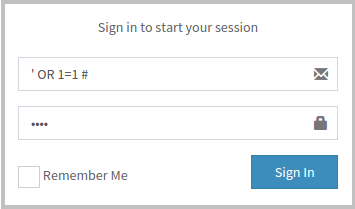
\includegraphics[width=0.5\textwidth]{img/sql_injection.png}
          \caption{Une tentative d'injection SQL sur un formulaire de contact}
          \label{fig:sql_injection}
        \end{figure}

      \paragraph{Injection JS}

        Le JavaScript est du code interprété sur le navigateur du client. Placé dans le document HTML, il sera exécuté par le navigateur. Par exemple, un petit malin peut créer un utilisateur contenant du code JavaScript comme nom de famille.

        \begin{scriptsize}
          \begin{lstlisting}[language=html, caption={Un exemple d'injection SQL}]
          <script>alert('Pwned')</script>
          \end{lstlisting}
        \end{scriptsize}

        Alors sur chaque page ou son nom sera affiché, le code sera exécuté. Heureusement, Rails nous protège directement de cela en échappant les caractères.

      \paragraph{Attaque par force brute}

        Il s'agit d'une attaque très facile à mettre en place. Il s'agit de tenter de se connecter plusieurs fois en utilisant un login et un dictionnaire de mots de passe.

        Dans mon cas, j'ai utilisé la bibliothèque \href{https://github.com/binarylogic/authlogic}{Authlogic} qui stocke le nombre de tentative de connections échouées dans la base de données. Ainsi, une fois 3 tentatives dépassées, le compte est bloqué et il n'est plus possible de se connecter avec le login.

    \subsection{Les failles les plus récentes}

      Des failles de sécurités sont découvertes tous les jours. Heureusement pour nous, une organisation les répertories. Ces vulnérabilités sont identifiées par un identifiant CVE\footnote{Common Vulnerabilities and Exposures}.

      \href{https://github.com/rubysec/ruby-advisory-db}{Ruby Advisory Database} est une base de données communautaire qui s'appuie sur ces CVE. Elle repertories les bibliothèques Ruby vulnérables à ces CVE. Des outils existent pour vérifier automatiquement que notre application n'utilise pas un bibliothèque vulnérable: \href{https://github.com/rubysec/bundler-audit}{Bundler Audit}.

      \href{https://github.com/rubysec/bundler-audit}{Bundler Audit} s'utilise très facilement:

      \begin{scriptsize}
        \begin{lstlisting}[language=bash]
        $ bundle audit
        Name: actionpack
        Version: 3.2.10
        Advisory: OSVDB-91452
        Criticality: Medium
        URL: http://www.osvdb.org/show/osvdb/91452
        Title: XSS vulnerability in sanitize_css in Action Pack
        Solution: upgrade to ~> 2.3.18, ~> 3.1.12, >= 3.2.13
        \end{lstlisting}
      \end{scriptsize}


  \section{Audit de sécurité}

    \subsection{Vérifier les ports ouverts}

      La première étape pour un hacker est la \textbf{reconnaissance de la cible}. Cette étape consiste à obtenir le maximum d'informations sur la victime. Nous devons donc cacher le plus d'informations possible à propos de notre serveur.

      Une des information facile à obtenir pour un hacker est les port ouverts sur le serveur. Les ports sont en quelques sortent des portes ouvertes sur le réseaux.

      Donc, dans un premier temps, j'ai simplement effectué un scan des ports sur mon serveur\footnote{Malgré sur ce qu'on peut entendre, le scan de port est tout à fait légal. \url{http://www.infond.fr/2010/09/legalite-du-scan-de-port.html}} avec \verb|nmap|\footnote{NMAP est un scanner de port} (voir listing \ref{lst:nmap})

      \begin{scriptsize}
        \begin{lstlisting}[language=bash, caption={Un san des port sur le serveur d'iSignif en novembre 2018}, label={lst:nmap}]
        $ sudo nmap isignif.fr -A

        Starting Nmap 7.60 ( https://nmap.org ) at 2018-11-16 11:25 CET
        Nmap scan report for isignif.fr (51.75.24.68)
        ...
        PORT     STATE    SERVICE      VERSION
        21/tcp   open     tcpwrapped
        22/tcp   open     ssh          OpenSSH 7.6p1 Ubuntu 4ubuntu0.1 (Ubuntu Linux; protocol 2.0)
        ...
        80/tcp   open     http         Apache httpd 2.4.29
        ...
        443/tcp  open     ssl/ssl      Apache httpd (SSL-only mode)
        ...
        Running (JUST GUESSING): Linux 3.X|4.X (86%), FreeBSD 6.X (85%)
        ...
        \end{lstlisting}
      \end{scriptsize}

      On voit donc que beaucoup d'informations ressortent du scan comme:

      \begin{itemize}
        \item l'utilisation d'OpenSSH port 22
        \item l'utilisation d'Apache HTTPD port 22 / 443
      \end{itemize}

      NMAP nous fournis aussi le numéro de la version des logiciels utilisés. Cela peut servir à trouver des vulnérabilités. Je vous montrerai comment j'ai masqué certains de ses informations lors de la sous-section \ref{subsec:change_ports}.

    \subsection{Réalisation d'un scan de vulnérabilité}

      Afin de connaître les vulnérabilité de mon installation, j'ai décidé de faire un scan de vulnérabilité en utilisant \href{https://www.metasploit.com/}{Metasploit}\footnote{Metasploit Framework est un logiciel écrit en Ruby permettant le développement et l’utilisation d'exploit. Les exploits sont des vulnérabilités qui permettent d’exécuter du code sur une machine distante.} et \href{http://www.openvas.org/}{OpenVAS}\footnote{OpenVAS est un scanner de vulnérabilités libre issu du fork de Nessus.}.

      Le scan de vulnérabilité est illégal à moins que le serveur nous appartienne ou bien qu'une autorisation du propriétaire est donné. Dans mon cas, le serveur m’appartiens.

      OpenVAS s'appuie sur les \href{https://cve.mitre.org/}{CVE (Common Vulnerabilities and Exposures)}. Il s'agit d'une base de données des vulnérabilités connues.

      Plusieurs types de scan sont possibles, j'ai choisis d'utiliser le plus complet, qui est aussi le plus long. J'ai donc obtenu le résultat que l'on peu voir figure \ref{fig:openvas_report} (le rapport complet est disponible annexe \ref{openvas_report}).

      \begin{figure}
        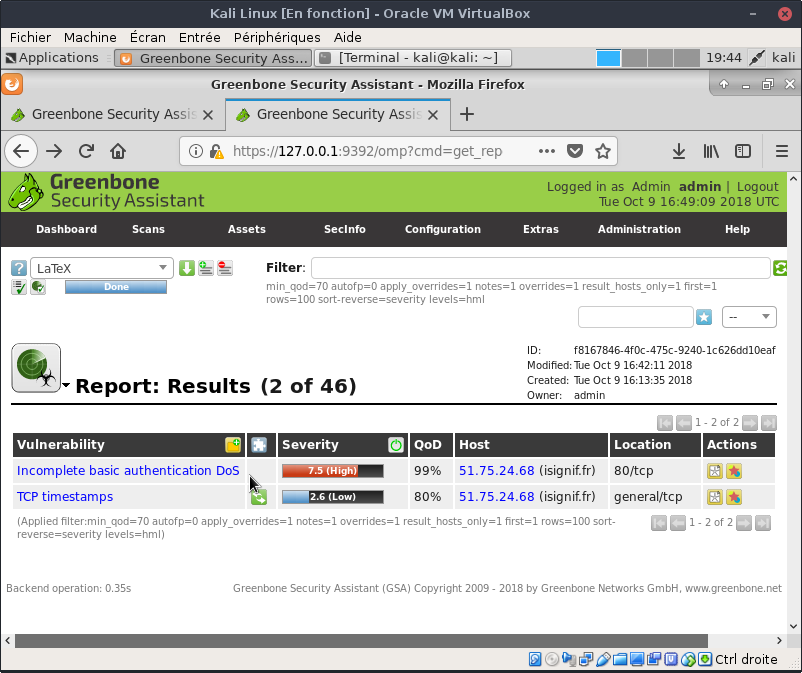
\includegraphics[width=\linewidth]{img/kali_openvas_report.png}
        \caption{Capture d'écran du rapport de scan d'OpenVAS}
        \label{fig:openvas_report}
      \end{figure}

      On peut voir que globalement mon serveur possède peu de vulnérabilités. Ceci est sûrement du au fait que je met à jours les paquets quotidiennement et que donc, les logiciels sont à jours.


  \section{Sécurité du serveur}

    Sécuriser un serveur est un travail à part entière qui nécessite beaucoup compétences. De plus, absolument personne ne peut se narguer d'être invulnérable aux tentatives d'attaques. Je n'ai pas la prétention d'être un expert en sécurité donc il s'agit ici de mettre en places les protections de base.

    \subsection{Utilisation du protocole HTTPS}

      Le \href{https://fr.wikipedia.org/wiki/HyperText_Transfer_Protocol_Secure}{protocole HTTPS} permet de chiffrer les communications entre le client et le serveur. Cela garantie que les informations qui transitent ne peuvent pas être lues par un attaquant. Ainsi, on protège les identifiants qui transite lorsqu'un utilisateur connecté.

      Auparavant, il fallait souvent payer une entreprise qui garantissait la validité de la clé de chiffrement. L'activer se fait  désormais très facilement grâce à \href{https://letsencrypt.org/}{Let's encrypt} qui est totalement gratuit!

      J'ai donc pu l'installer très facilement avec \href{https://certbot.eff.org/}{Certbot}, un outil qui génère le certificat pour nous et s’occupe même de mettre la configuration Apache à jour.

      \begin{scriptsize}
        \begin{lstlisting}[language=bash]
        $ sudo certbot --apache
        \end{lstlisting}
      \end{scriptsize}

      C'est donc un petit geste mais celui-ci à des répercutions sur la confiances accordée par nos utilisateur et même sur le référencement\footnote{Google à annoncé en aout 2014 que le protocole HTTPS serait pris en compte dans l'algorithme de positionnement. \url{https://webmaster-fr.googleblog.com/2014/08/le-protocole-https-en-tant-que-facteur.html}}.

    \subsection{Groupe sudo}

      Comme je l'ai évoqué plus haut, j'ai déjà crée un utilisateur spécifique pour l'application que j'ai rajouté dans le groupe des \verb|sudoers|. Une des actions qui peut être mis en place facilement est de supprimer cet utilisateur du groupe \verb|sudo|. Ceci permet d'éviter l’élévation des privilèges\footnote{Un des premier objectif d'un hacker va être de vouloir obtenir des privilèges plus élevé afin de pouvoir effectuer des actions ayant de plus grandes conséquences}.

    \subsection{Modifier le port par défaut}\label{subsec:change_ports}

      En regardant les logs d'un serveur, on peut remarquer une quantité importante de tentative de connexion SSH\footnote{Le protocole SSH permet de se connecter à distance à un ordinateur}. Ceci est du au fait que beaucoup de hacker ont mis au point des scripts qui tentent de se connecter en utilisant des dictionnaires de mots de passe.

      Par défaut, le port utilisé est le port 22.

        %TODO

    \subsection{Blacklister les tentatives de connexions}

      Comme je l'expliquait plus haut, beaucoup de hacker tentent de se connecter au serveur via la protocole SSH. De la même manière que pour les appels téléphonique, il est possible de bloquer ces tentatives.

       \href{https://www.fail2ban.org/wiki/index.php/Main_Page}{Fail2ban} est un petit utilitaire écrit en Python qui va s’occuper d'analyser les logs du serveur. Il va donc mettre sur liste noir les adresses IP qui ont tenté de se connecter plusieurs fois avec un mot de passe erroné.




\chapter{Amélioration continue}

  \section{RGPD}

    2018 fut l'année de la mise en place de la RGPD\footnote{Règlement général sur la protection des données}. Entrée en vigueur le 25 mai, ce texte réglementaire européen couvre, entre autres, le traitement des données personnelles\footnote{Les données personnelle sont toutes les données qui permettent d'identifier quelqu'un}.

    Les principales nouveautés qu'apporte la RGPD sont:

    \begin{itemize}
      \item le droit à l'oubli
      \item le droit à la portabilité des données
      \item le droit à l'opposition de toute opération marketing
      \item le droit à la rectification des données de l'utilisateur
      \item le droit d'accès à toutes les données de l'utilisateur
    \end{itemize}

    Il faut qu'il y ait un Délégué à la Protection des Données (DPD).

    % pompé sur https://bohzo.developpez.com/rgpd-guide-pratique-developpeurs

    Dans mon cas, les principales obligations qui m'incombent sont les suivantes:

    \begin{itemize}
      \item l'utilisateur doit pouvoir effacer toutes les données de l'application qui le concerne \href{Chapitre 3, Article 17}{https://gdpr-info.eu/art-17-gdpr/}
      \item l'utilisateur doit pouvoir conn
      \item nous devons stocker le minimum de données possible
    \end{itemize}


    \subsection{Oubliez-moi}\label{subsec:forget-me}

      \href{L'article 17 de la RGPD}{https://gdpr-info.eu/art-17-gdpr/} nous oblige à implémenter une fonctionnalité \textquote{Oubliez-moi}. Celle-ci doit permettre à l'utilisateur d'effacer toutes ses données immédiatement. La ou cela se complique, c'est que la RGPD nous oublige aussi à demander la suppression des données chez des fournisseurs tiers. Ainsi, si nous utilisons des services externes\footnote{Salesforce, Hubspot, Twitter, ou tout autre fournisseur de service cloud} il faut accéder à leur API afin de demander la suppression.

      La difficulté de cette fonctionnalité est de supprimer les données liées à l'utilisateur sans impacter les données qui sont liées aux autres utilisateurs.

      \subsubsection{Exemple avec un huissier de justice}

        Concrètement, cela signifie que lorsqu'un huissier de justice décide de supprimer son compte, il faut:

        \begin{itemize}
          \item supprimer son compte et ses données (logique)
          \item supprimer toutes ses factures
          \item supprimer les significations\footnote{L'acte de présenter en main propre un acte de signification à quelqu'un} qu'il a effectué
        \end{itemize}

        Cependant je ne peux pas supprimer les significations puisqu'elles doivent être conservée pour l'avocat qui a demandé la signification de son acte.

        C'est pour cela que j'ai préféré l'\textbf{anonymisation} des données.

        Comme je l'expliquait section \ref{sec:tdd}, je suis un évangéliste du \textit{Test Driven Development}. J'ai donc commencé par construire le test.

        \begin{scriptsize}
          \begin{lstlisting}[language=ruby]
          # test/models/bailiff_test.rb
          require 'test_helper'

          class BailiffTest < ActiveSupport::TestCase
            # ...

            test 'should anonymize and not destroy record' do
              old_user = @bailiff.as_json

              # on verifie que l'huissier n'est pas supprime en base
              assert_no_difference('Bailiff.count') { @bailiff.destroy }

              # on verifie que tous les champs suivants on ete modifies
              %i[email firstname lastname siret company_name town zip_code address_2 address_1].each do |field|
                assert_not_equal old_user[field], @bailiff.send(field)
              end

              # et pour terminer, un champ 'deleted' a dut etre passe a 'true'
              assert @bailiff.deleted
            end
          end
          \end{lstlisting}
        \end{scriptsize}


        \textit{ActiveRecord} (l'ORM\footnote{Un ORM fait interface entre le code et la base de données, voir \href{https://fr.wikipedia.org/wiki/Mapping_objet-relationnel}{la définition complète sur Wikipedia}} de Ruby on Rails). J'ai donc simplement surchargé la méthode \verb|destroy| et utilisé la librairie \verb|Faker|\footnote{Il s'agit d'une librairie utilisée pour générer des fausse données en tout genre}:

        \begin{scriptsize}
          \begin{lstlisting}[language=ruby]
          # app/models/user.rb
          class User < ApplicationRecord

            # ...

            def destroy
              # ...

              update_attributes(
                email: new_email,
                firstname: Faker::Name.first_name,
                lastname: Faker::Name.last_name,
                siret: Faker::Company.french_siret_number,
                # ...
                deleted: 1
              )

              save
            end
          end
          \end{lstlisting}
        \end{scriptsize}

        Et voilà, la mise en conformité est faite. L'huissier ou l'avocat pourra supprimé son compte et les données seront conservées. En revanche, il sera impossible de retrouver l'utilisateur correspondant à ces données.

    \subsection{Cookies}

        %TODO

    \subsection{Chiffrement des données}

        %TODO

  \section{Déploiement continue}\label{sec:deployments}

    Afin d'être le plus réactif possible, j'ai voulu mettre en place un outil afin d'automatiser les mises en production. Cela est un énorme avantage car il permet de mettre en ligne un correctif ou une évolution très rapidement. De plus, automatiser permet de réduire le risque de l'erreur humaine (\href{https://www.reddit.com/r/webdev/comments/5rd79m/gitlab_employee_just_ran_rm_rf_on_their/}{et cela est vite arrivé}...).

    Pour cela, j'ai utilisé la librairie \href{https://capistranorb.com}{Capistrano}. Capistrano est un outil écrit en Ruby qui permet d'automatiquement le déploiement en s'appuyant sur Git (rappelez vous de mon utilisation de Git Flow section \ref{sec:git}). Il va donc:

    \begin{itemize}
      \item Cloner le répertoire Git afin de récupérer la dernière version du code source
      \item Lancer les modifications sur la base de données
      \item Minifier\footnote{Il s'agit de concateiner les fichiers texte en un seul afin de réduire le nombre de requête HTTP et d'améliorer la vitesse de chargement} les fichiers Javascript et CSS
      \item Faire des liens symboliques sur les documents que les utilisateurs ont envoyés sur le serveur
    \end{itemize}

    La librairie se met en place très facilement, voici un extrait de ma configuration

    \begin{scriptsize}
    \begin{lstlisting}[language=ruby]
    # config/deploy.rb

    set :application, "iSignif"
    set :repo_url, "http://git.rousseau-alexandre.fr/iSignif/Website.git"
    append :linked_files, 'config/database.yml' , 'config/initializers/secret_token.rb', 'config/secrets.yml'
    append :linked_dirs, 'public/uploads'
    \end{lstlisting}
    \end{scriptsize}

  \section{Retours des utilisateurs}\label{sec:feedback}

    \subsection{Service après vente}

        %TODO

    \subsection{Témoignages}

        %TODO

\chapter{Marketing}

  \section{Référencement}

  \section{Vidéo de démonstration}

  \section{Création d'une campagne de publicité avec LinkedIn}

    Notre produits s’adressant aux professionnels, nous avons choisi le réseau social LinkedIn\footnote{LinkedIn est un réseau social entre professionnels} pour promouvoir notre plateforme.

    Le but était donc de toucher principalement:

    \begin{itemize}
        \item les huissiers pour qu'ils rejoignent le réseaux iSignif
        \item les avocats pour qu'ils signifient des actes sur notre site
    \end{itemize}

    \subsection{Les types de publicité}

      LinkedIn propose trois types de publicité:

      \begin{itemize}
        \item Sponsored Content, la publicité arrive directement dans le fil d'actualité de l'utilisateur
        \item Text Ads, la publicité est plus discrète et ce place sur le côté de l'application
        \item Sponsored InMail, la publicité est envoyée directement par chat et permet donc de démarrer une discussion avec l'utilisateur s'il le souhaite
      \end{itemize}

      \begin{figure}
        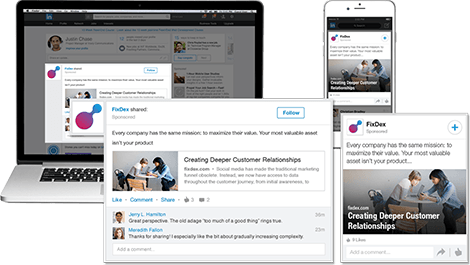
\includegraphics[width=\linewidth]{img/linkedin_sponsored_content.png}
        \caption{la publicité de type Sponsored Content propose un contenu riche}
        \label{linkedin_sponsored_content}
      \end{figure}

      Pour la campagnes à destination des avocats, nous avons décidé d’utiliser le modèle Sponsored Content. Comme le montre la figure \ref{linkedin_sponsored_content}, ce modèle à l'avantage de proposer un contenu riche grâce à une image et à un lien qui redirige directement sur le site. De plus, LinkedIn offre la possibilité de cibler l'audience et donc d'obtenir une audience de qualité.

      %TODO

\chapter{Conclusion}

  \section{Apports professionnels}

    Les apports professionnels d'une telle expérience sont évidents. Au delà de mettre en avant une expérience professionnelle de plus, j'ai énormément appris.

    Tout d'abord, en étant le référent technique d'un projet, j'ai eu l'occasion de choisir les technologies que je voulais utiliser. J'ai donc pu mettre en place un environnement ou je me sentais à l'aise et ou je prenais du plaisir à travailler.

    Ensuite, cette expérience à été pour moi l'opportunité de découvrir un autre rôle au sein d'un société.

    %TODO

  \section{Apports personnels}

    %TODO

  \section{Perspectives}

    %TODO


    \begin{appendix}
        \chapter{Rapport de scan OpenVAS}
        \label{openvas_report}
        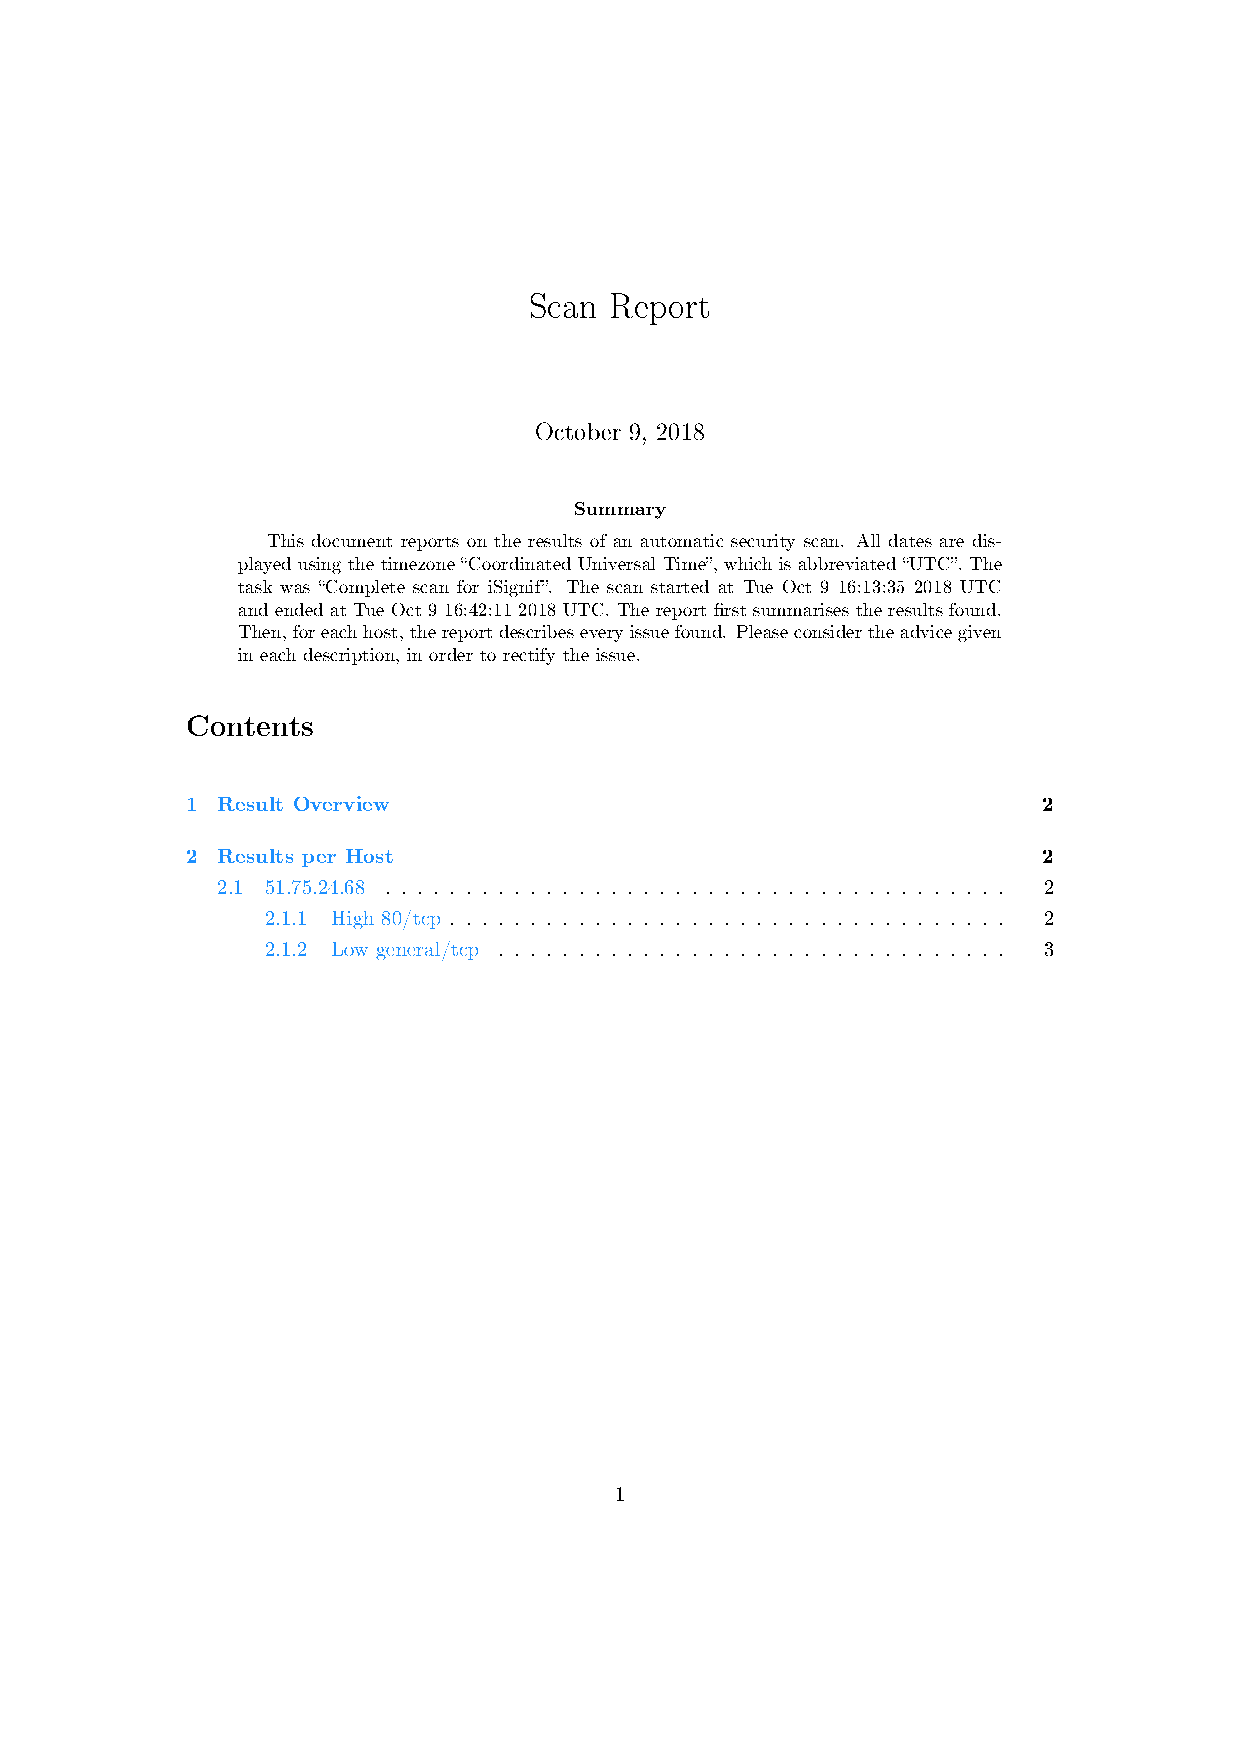
\includepdf[pages=-]{annexes/openvas_report.pdf}
    \end{appendix}

\end{document}
